\section{Methods}
DBSCAN has two main parameters epsiolon($\epsilon$) and minPoint.
$\epsilon$ defines the distance to search for object and minPoint defines minimum number of objects to be dense. there are three type of point in DBSCAN:
\begin{itemize}
	\item Core
	\item Border
	\item Noise
\end{itemize}
Core is a point which has at least p point in distance d. Border is a point that has at lease one core point at distance d, and Noise is a point that there is less than p point in distance d or in other word it is not core nor border.
\textbf{Reachability} means if a point distance is less than $\epsilon$ it is reachable.
\textbf{Connectivity} means when two points are connected through reachable dense space. you can see an example in figure \ref{fig:dbscan-example}.
\begin{figure}[h]
	\centering
	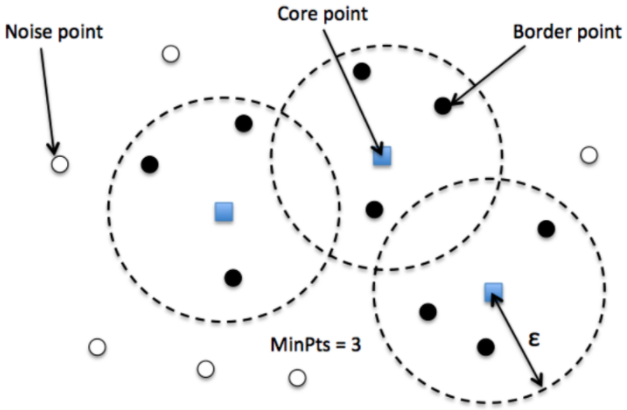
\includegraphics[width=0.9\linewidth]{figures/DBSCAN-example}
	\caption{Example of DBSCAN and its definitions\cite{kdnuggetsDBSCAN}.}
	\label{fig:dbscan-example}
\end{figure}
the method can be summery in algorithm \ref{alg:alg1}.

\begin{algorithm}
	\KwIn{$\epsilon$, MinPoint, DistanceFunction, DB}
	set $ X_{un} = X$ \\
	set $ m = 0 $ \tcp*{Cluster counter}
	\While{$ X_{un} \neq \O$}{
		Arbitrarily select a $ x \in X_{un}$ \\
		\If{$ x $ \text{is a noncore point}}{
			Mark $ x $ as a noise point\\
			$ X_{un} = X_{un} - \{x\} $\\
		}
		\If{$ x $ is a core point}{
			$ m = m + 1 $\\
			Determine all density-reachable points in $ X $ from $ x $\\
			Assign $ x $ and the previous points to the cluster $ C_m $\\
			The border points that may have been marked as noise are also assigned to $ C_m $\\
			$ X_{un} = X_{un} - C_m $\\
		}
	}
	\caption{DBSCAN pseudocode}
	\label{alg:alg1}
\end{algorithm}